\documentclass[12pt]{article} \usepackage{COSC420style} \usepackage{soul}
\usepackage{booktabs}
\usepackage{verbatim}
\usepackage{hyperref}
\usepackage{graphicx}
\usepackage{subcaption}
\papercode{COSC420}

\title{Transformer based language model}

\author{Jake \textsc{Norton}} \studentid{5695756}

\reportdate{\today}

\begin{document}

\maketitle

\section{Introduction}

Transformer-based models have revolutionized the field of natural language
processing, offering unprecedented advancements in text generation tasks. These
models are lauded for their ability to understand and generate complex language
patterns, making them highly effective for a variety of applications, from
chatbots to literary analysis. Despite their widespread success, transformer
models often encounter challenges, particularly when applied to smaller,
stylistically unique datasets. This report explores the performance of such
models, specifically focusing on their capability to generalize and produce
novel text. Many of the decisions made here were close to arbitrary in nature
due to time constraints, and I did not get to explore as much as I would have
liked. However, I do believe that the models created are still adequate at
creating text that is at least interesting. For this study, the datasets
comprised the complete texts of two distinct books, including the voluminous and
stylistically rich War and Peace. Using the entirety of these books provided a
higher volume of data, although it introduced a potential bias towards the
themes, style, and vocabulary prevalent in War and Peace. This was a conscious
trade-off, made in the hope that the larger volume of data would enhance the
model’s performance, even if potentially skewing it towards the narrative style
and vocabulary of War and Peace. This skew could influence the model's ability
to generate universally applicable text, potentially limiting its generalization
capabilities outside the specific contexts of the used texts. Despite this
limitation, the aim was to evaluate how well the model could adapt and generate
text that was not only syntactically coherent but also rich in varied linguistic
expressions and themes derived from the comprehensive datasets.

\section{Task 1: Tok2Vec Encoder}

\subsection{Methodology}

Word2vec embeddings can be created using two primary approaches: Skip-gram (SG) and Continuous Bag
of Words (CBOW). These methods are essentially opposites; CBOW predicts a word based on the context
of surrounding words, while Skip-gram, conversely, predicts the surrounding context from a given
word. CBOW is effective for identifying common links among frequently used words, making it ideal
for smaller datasets where the focus is on simpler relationships that require less data to discern.
However, the method's tendency to average context can lead to a less detailed understanding. In
contrast, Skip-gram excels in capturing more complex relationships but requires more data and longer
training times. Each position in the context window must be trained separately, unlike CBOW, which
integrates all context simultaneously.

I was under the impression that the general consensus holds Skip-gram to be
better suited for larger datasets, while CBOW can still perform well with
smaller ones. However, I did not find any conclusive studies to substantiate
this, although it's possible I may have overlooked some. I chose to use
Skip-gram for its potential to uncover interesting patterns, despite the
limitations of our dataset. I also hypothesized that Skip-gram might perform
better on smaller datasets given sufficient time, as it processes the data
multiple times, equal to the size of the context window. The context window size
is important as it determines how many words around a target word are considered
when forming predictions, directly influencing the model’s ability to grasp
broader textual contexts and nuances. Unfortunately, the exploration process was
constrained by early corruption in my token-to-vector models. To streamline the
process, I saved the encoded vectors of the entire corpus for repeated use,
which significantly reduced processing time. However, at some point, I believe
the saved dataset became corrupted, as the predictions consistently returned the
tokens \textit{i}, \textit{\ae}, \textit{=}. Initially, the t-SNE plots
suggested that the models were successfully clustering semantically similar
words, so I did not realize there was a corruption issue until I began training
the transformer models. Once I reencoded the dataset, this issue was resolved in
all versions of the model.

\begin{table}[htbp]
	\centering
	\caption{Frequency of Words with Different Context Window Sizes}
	\label{tab:word_frequencies}
	\begin{tabular}{cccccc}
		\toprule
		\multicolumn{2}{c}{Context window size 3} & \multicolumn{2}{c}{Context window size 4} & \multicolumn{2}{c}{Context window size 5}                                                \\
		\cmidrule(r){1-2} \cmidrule(lr){3-4} \cmidrule(l){5-6}
		Token                                     & Probability                               & Token                                     & Probability & Token            & Probability \\
		\midrule
		\textbackslash s                          & 0.0655                                    & \textbackslash s                          & 0.0673      & \textbackslash s & 0.0911      \\
		the                                       & 0.0322                                    & ,                                         & 0.0329      & the              & 0.0446      \\
		,                                         & 0.0301                                    & the                                       & 0.0315      & ,                & 0.0419      \\
		and                                       & 0.0205                                    & and                                       & 0.0216      & .                & 0.0272      \\
		.                                         & 0.0185                                    & .                                         & 0.0210      & and              & 0.0260      \\
		of                                        & 0.0176                                    & of                                        & 0.0210      & of               & 0.0238      \\
		to                                        & 0.0169                                    & to                                        & 0.0150      & to               & 0.0175      \\
		a                                         & 0.0114                                    & in                                        & 0.0112      & a                & 0.0135      \\
		in                                        & 0.0100                                    & a                                         & 0.0107      & in               & 0.0121      \\
		his                                       & 0.0086                                    & his                                       & 0.0084      & his              & 0.0097      \\
		was                                       & 0.0076                                    & was                                       & 0.0075      & was              & 0.0083      \\
		that                                      & 0.0073                                    & with                                      & 0.0070      & with             & 0.0076      \\
		he                                        & 0.0067                                    & that                                      & 0.0063      & that             & 0.0071      \\
		her                                       & 0.0064                                    & he                                        & 0.0061      & he               & 0.0069      \\
		with                                      & 0.0064                                    & had                                       & 0.0053      & her              & 0.0063      \\
		'                                         & 0.0061                                    & at                                        & 0.0053      & had              & 0.0059      \\
		had                                       & 0.0052                                    & on                                        & 0.0051      & at               & 0.0056      \\
		at                                        & 0.0050                                    & her                                       & 0.0051      & '                & 0.0054      \\
		it                                        & 0.0046                                    & '                                         & 0.0049      & on               & 0.0052      \\
		"                                         & 0.0045                                    & for                                       & 0.0041      & "                & 0.0051      \\
		\bottomrule
	\end{tabular}
\end{table}

Regarding the context window for the model, I found that a size below 3 yielded poor results in
prediction tests. I experimented with sizes up to 5, but choosing between 3, 4, and 5 proved
challenging. The larger the context window, the more it prioritized punctuation, as shown in
Table~\ref{tab:word_frequencies}. Eventually, I opted for a context window of 4, aiming to balance
the difference and reduce training time. I was ultimately satisfied with the punctuation versus text
balance, though the model still occasionally struggles with quotations. Models with a context window
of 4 generally showed a nicely distributed clustering of semantically similar words such as "would,
should, could, must, shall."

To determine the vocabulary size, I performed a rough count of unique words using a series of Bash
commands\footnote{bash command: \texttt{tr '[:upper:]' '[:lower:]' < combined\_books\_text | tr -d
'[:punct:]' | tr ' ' '\textbackslash{}n' | sort | uniq | wc -l}, in part crafted by ChatGPT},
resulting in approximately 25,000 words. However, this count included many duplicates or
near-duplicates due to punctuation, as demonstrated by the list of variations of the word 'your'.

\begin{itemize}
	\item   ‘your
	\item   “your
	\item   your
	\item   “you’re
	\item   you’re
\end{itemize}

To maximize coverage while managing memory and model size limitations, I capped the token count at
5,000, reasoning that if ChatGPT operates effectively with around 50,000 unique tokens, 10\% should
be sufficient for a corpus of this size.

I also explored various sizes for the hidden layer dimensions, ranging from 32 to 512. Limited
testing made it difficult to determine the best size quantitatively, though it was evident that
dimensions of 32 and 64 were insufficient, as they resulted in a noticeable skew in the graphical
outputs. While t-SNE reduces dimensionality and may not make a linear skew inherently problematic,
my interpretation was that such skewness indicated a simpler embedding representation.

\subsection{Hyperparameters}
\begin{itemize}
	{\small
	\item \textbf{Context Window}: 4
	\item \textbf{Hidden Layer Dimension}: 256
	\item \textbf{Vocab Size}: 5000
	      }
\end{itemize}

\subsection{Architecture}
\begin{table}[htbp]
	\centering
	\caption{Model Architecture Details} % Add an appropriate caption here
	\label{tab:model_architecture} % Add a descriptive label
	\begin{tabular}{lcc} % Corrected alignment settings; use 'l' for left, 'c' for center
		\toprule
		Layer (type)       & Shape & Params    \\
		\midrule
		input (InputLayer) & 5000  & 0         \\
		embedding (Dense)  & 256   & 1,280,000 \\
		output (Dense)     & 5000  & 1,285,000 \\
		\bottomrule
		Total params: 2,565,000
	\end{tabular}
\end{table}


\begin{figure}[htbp]
	\centering
	\begin{subfigure}[b]{0.45\textwidth}
		\includegraphics[width=\textwidth]{./figures/dim_32_ctx_1_embedding.pdf}
		\caption{neurons: 32, context window of 1}
		\label{fig:32_1}
	\end{subfigure}
	\begin{subfigure}[b]{0.45\textwidth}
		\includegraphics[width=\textwidth]{./figures/dim_32_ctx_4_embedding.pdf}
		\caption{neurons: 32, context window of 4}
		\label{fig:32_4}
	\end{subfigure}
	\newline % starts a new line
	\begin{subfigure}[b]{0.45\textwidth}
		\includegraphics[width=\textwidth]{./figures/dim_64_ctx_3_embedding.pdf}
		\caption{neurons: 64, context window of 3}
		\label{fig:64_3}
	\end{subfigure}
	\begin{subfigure}[b]{0.45\textwidth}
		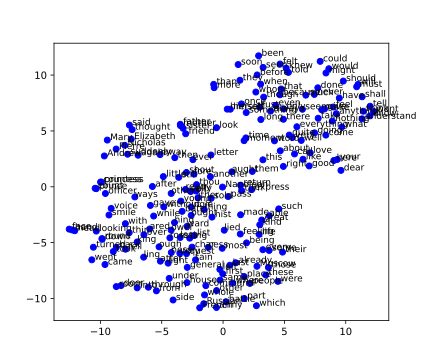
\includegraphics[width=\textwidth]{./figures/dim_64_ctx_5_embedding.pdf}
		\caption{neurons: 64, context window of 5}
		\label{fig:64_5}
	\end{subfigure}
	\caption{t-SNE plots of embedding space with varying sizes of neurons and context
		windows}
	\label{fig:small_embeddings}
\end{figure}

\begin{figure}[htbp]
	\centering
	\begin{subfigure}[b]{0.45\textwidth}
		\includegraphics[width=\textwidth]{./figures/dim_64_ctx_4_embedding.pdf}
		\caption{neurons: 64, context window: 4}
		\label{fig:64_4}
	\end{subfigure}
	\hfill % Add horizontal space between the first and second subfigures on the same row
	\begin{subfigure}[b]{0.45\textwidth}
		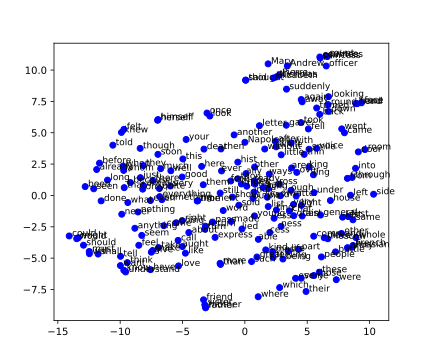
\includegraphics[width=\textwidth]{./figures/dim_128_ctx_4_embedding.pdf}
		\caption{neurons: 128, context window: 4}
		\label{fig:128_4}
	\end{subfigure}
	\newline % Starts a new line for the next row: subfigures
	\begin{subfigure}[b]{0.45\textwidth}
		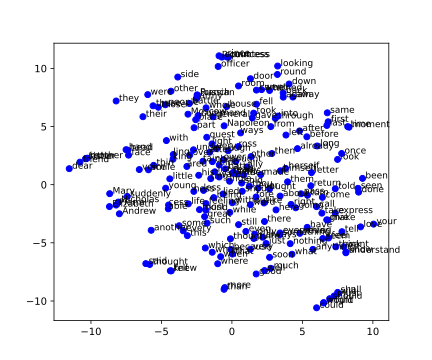
\includegraphics[width=\textwidth]{./figures/dim_256_ctx_4_embedding.pdf}
		\caption{neurons: 256, context window: 4}
		\label{fig:256_4}
	\end{subfigure}
	\hfill % Add horizontal space between the first and second subfigures on the same row
	\begin{subfigure}[b]{0.45\textwidth}
		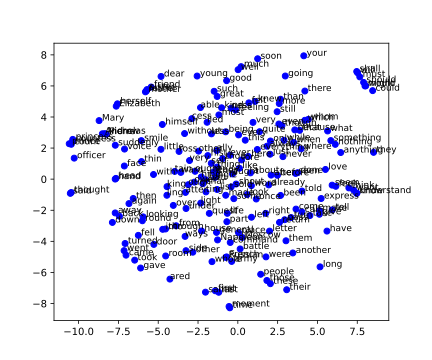
\includegraphics[width=\textwidth]{./figures/dim_512_ctx_4_embedding.pdf}
		\caption{neurons: 512, context window: 4}
		\label{fig:512_4}
	\end{subfigure}
	\caption{t-SNE plots of embedding space with varying sizes of neurons and context windows}
	\label{fig:larger_embeddings}
\end{figure}


\section{Task 2: Transformer-based Text Prediction}

\subsection{Methodology}

Utilizing the provided transformer, I modified the model to accommodate my
256-dimensional embeddings and to accept one-hot vectors as inputs. Due to time
constraints and observing patterns in the training behavior, I limited the
training to a single epoch. As detailed in Section~\ref{sec:5_epoch_val},
extending training didn’t improve validation accuracy; instead, it worsened the
validation loss. Moreover, increases in training accuracy without corresponding
improvements in validation accuracy suggested a propensity for overfitting. This
often resulted in the model replicating text verbatim, particularly from War and
Peace.

I should note that the stagnation in validation accuracy and overall model
generalization might be attributed to an excessively high learning rate, which
could cause the model to repeatedly settle into local minima. In the final
setup, I omitted the validation split and utilized the entire dataset. The
quality of the model's outputs was then assessed more qualitatively, rather than
relying strictly on quantitative metrics.

\begin{table}[htbp]
	\centering
	\caption{Performance Metrics for Different Configurations}
	\label{tab:performance_metrics}
	\begin{tabular}{cccccc}
		\toprule
		\multicolumn{6}{c}{Transformer with Embeddings}                                                                  \\
		\midrule
		\textbf{Attention Heads} & \textbf{Transformer Layers} & \textbf{DFF} & \textbf{Loss} & \textbf{Masked Accuracy} \\
		4                        & 4                           & 256          & 2.8427        & 0.4136                   \\
		4                        & 4                           & 512          & 2.6718        & 0.4373                   \\
		4                        & 6                           & 256          & 2.6647        & 0.4402                   \\
		4                        & 6                           & 512          & 2.4718        & 0.4695                   \\
		16                       & 4                           & 256          & 2.3300        & 0.4995                   \\
		16                       & 4                           & 512          & 2.2095        & 0.5197                   \\
		16                       & 6                           & 256          & 2.0522        & 0.5551                   \\
		16                       & 6                           & 512          & 1.9590        & 0.5725                   \\
		\midrule
		\multicolumn{6}{c}{Transformer using One-hot Representation}                                                     \\
		\midrule
		4                        & 4                           & 256          & 2.2441        & 0.5154                   \\
		4                        & 4                           & 512          & 2.1719        & 0.5289                   \\
		4                        & 6                           & 256          & 2.0241        & 0.5586                   \\
		4                        & 6                           & 512          & 1.9068        & 0.5823                   \\
		16                       & 4                           & 256          & 1.6985        & 0.6311                   \\
		16                       & 4                           & 512          & 1.6726        & 0.6358                   \\
		16                       & 6                           & 256          & 1.4977        & 0.6802                   \\
		16                       & 6                           & 512          & 1.4662        & 0.6856                   \\
		\bottomrule
	\end{tabular}
\end{table}

\section*{Model Validation Results from 5 Epochs}

\label{sec:5_epoch_val}
\subsection*{Embedded Model}
\begin{tabular}{cccc}
	\toprule
	Epoch & Masked Accuracy & Val Loss & Val Masked Accuracy \\
	\midrule
	1     & 0.6024          & 8.5683   & 0.2430              \\
	2     & 0.8536          & 9.9641   & 0.2390              \\
	3     & 0.8941          & 10.4360  & 0.2372              \\
	4     & 0.9106          & 10.6708  & 0.2369              \\
	5     & 0.9202          & 10.7672  & 0.2373              \\
	\bottomrule
\end{tabular}

\subsection*{One Hot}
\begin{tabular}{cccc}
	\toprule
	Epoch & Masked Accuracy & Val Loss & Val Masked Accuracy \\
	\midrule
	1     & 0.7033          & 10.5074  & 0.2285              \\
	2     & 0.9168          & 11.5308  & 0.2275              \\
	3     & 0.9364          & 11.8598  & 0.2270              \\
	4     & 0.9448          & 11.8583  & 0.2263              \\
	5     & 0.9498          & 11.6422  & 0.2252              \\
	\bottomrule
\end{tabular}

\subsection{Model Architectures}
\begin{table}[htbp]
	\centering
	\caption{Detailed Comparison of Model Architectures}
	\label{tab:model_architectures}
	\begin{tabular}{lccc}
		\toprule
		\multicolumn{4}{c}{\textbf{Architecture Details}}                                                     \\
		\midrule
		                        & \textbf{Parameter}    & \textbf{Embedded Transformer} & \textbf{One Hot}    \\
		\midrule
		\textbf{Layer (type)}   & \textbf{Output Shape} & \textbf{Parameters}           & \textbf{Parameters} \\
		\midrule
		Fixed/One Hot Embedding & \(100 \times 256\)    & 0                             & 0                   \\
		Positional Encoding     & \(100 \times 256\)    & 0                             & -                   \\
		Dense                   & \(100 \times 256\)    & -                             & 1,280,256           \\
		Transformer Layer       & \(100 \times 256\)    & 790,016                       & 790,016             \\
		Transformer Layer 1     & \(100 \times 256\)    & 790,016                       & 790,016             \\
		Transformer Layer 2     & \(100 \times 256\)    & 790,016                       & 790,016             \\
		Transformer Layer 3     & \(100 \times 256\)    & 790,016                       & 790,016             \\
		Transformer Layer 4     & \(100 \times 256\)    & 790,016                       & 790,016             \\
		Transformer Layer 5     & \(100 \times 256\)    & 790,016                       & 790,016             \\
		Final Dense             & \(100 \times 5000\)   & 1,285,000                     & 1,285,000           \\
		\midrule
		\textbf{Total Params}   &                       & 6,025,096                     & 7,305,352           \\
		\bottomrule
	\end{tabular}
\end{table}

\section{Results}

In the following section, Section~\ref{sec:embedded_from_unseen}, the examples
illustrate significantly fewer direct copies of passages. Nevertheless, the
influence of the original texts is evident, albeit less directly replicated. I was disappointed to
find out that "The bloodstained smith" was not of its own making, though "torn
from his own wood" is, make of that what you will.

\subsection{Observations}

Deciding whether the one-hot or embedding-based model performs better presents a
complex challenge. The one-hot model seems more inclined to copy text directly,
as evidenced by pattern matches, indicating a potential struggle with
generalization. Conversely, the overall quality of output from both models
points to limited generalization capabilities. Familiarity with War and Peace
would likely enhance my ability to detect borrowed themes and characters,
further informing this comparison.

It’s also noteworthy that the overtrained embedding model handles punctuation
with notable proficiency; at a glance, its output might be mistaken for
well-composed prose. However, this appearance is deceptive, as much of the text,
particularly marked in red[\ref{sec:verbatimtext}], is lifted directly from the source material. This
tendency is even more pronounced in the one-hot model
	[\ref{sec:one_hot_over_training}], where the extent of
direct copying is arguably worse.

\subsubsection*{Bias}

The bias is obviously present in the model outputs. It is much more likely to
generate text with heavy \textit{inspiration} from War and Peace. As for whether
have a more balanced dataset would have improved the model overall is hard to
tell.

\subsubsection*{Further Work}

There are several additional experiments I would have liked to conduct if time had permitted, specifically:

\begin{itemize}
	\item A more comprehensive evaluation of similarities between the generated
	      output and the source material to better understand the model's ability
	      to innovate versus replicate.

	\item Investigation of various learning rates and optimizers to determine
	      whether rapid convergence was reaching a local minimum or if more
	      optimal minima could be achieved with a gentler learning rate.

\end{itemize}

\section{Conclusion}

To conclude, transformer-based models are powerful tools capable of generating
text that closely approximates human-like syntax, even when trained on small and
highly stylized datasets. However, these models face significant challenges in
generalizing their output. Due to the limited range of patterns they can learn,
there is a heightened risk of reproducing source text verbatim, particularly
when overtrained. Based on my testing, if the objective is to generate new, more
original text, the embedding-based model seems to have a distinct advantage, the
embedding space allows it produce novel content, whereas the one-hot model often
merely replicates existing text, functioning much like a cut-and-paste parrot.

% \section{Examples}
% \label{sec:verbatimtext}
% \subsection{generated text}
% prompt: check the logs \\
% \\
% {\footnotesize
% check the logs,  \textcolor{red}{and the air of a man who enjoys life and knows
% 	how to live,  he swayed to and fro with dignity,  offered surmises about the
% 	weather, or touched on questions of health, sometimes in russian and
% 	sometimes in very bad but self -  confident french;  then again,  like a man
% 	weary but unflinching in the fulfillment of duty,  he rose to see some
% 	visitors off and, stroking his scanty gray hairs over his bald patch,  also
% 	asked them to dinner.  sometimes on his way back from the anteroom he would
% 	pass through the conservatory and pantry into the large marble dining hall,
% 	where tables were being set out for eighty people;  and looking at the
% 	footmen,  who were bringing in silver and china, moving tables,  and
% 	unfolding damask table linen,  he would call dmítri vasílevich,  a man of good
% 	family and the manager of all his} family and the old friend of the creator,
% and was already regarding him where and spent most of the highest wisdom.  he
% was,  as a result of the one that danger,  was able to intensate the purposely
% coming with the emperor and colonel.  they were the same,  rostóv felt that the
% commander had not gone on for achievement and that something great many english
% were being held.  he turned away and waited for them,  asking him to come to
% rest.  the letters resounded the lectance tenor, having come up to the small and
% em denísov,  came up to dinner.  after he had been ordered for night at a time
% that night he had been prepared for the last two months,  and though he still
% his corps had quite lost in the village of battle,  as nevert

% \begin{verbatim}
% ('pride_matches', [])
% ('war_matches', ['the air of a man', 'air of a man who', 'of a man who enjoys',
% 'a man who enjoys life', 'man who enjoys life and', 'who enjoys life and knows',
% 'enjoys life and knows how', 'life and knows how to', 'and knows how to live,',
% 'knows how to live, ', ' he swayed to and', ' offered surmises about the',
% 'offered surmises about the weather,', 'surmises about the weather, ', '
% sometimes in russian and', 'sometimes in russian and sometimes', 'in russian and
% sometimes in', 'russian and sometimes in very', 'and sometimes in very bad',
% 'sometimes in very bad but', ' like a man weary', 'like a man weary but', 'a man
% weary but unflinching', 'man weary but unflinching in', 'the fulfillment of
% duty, ', ' he rose to see', 'he rose to see some', 'rose to see some visitors',
% 'to see some visitors off', 'see some visitors off and,', 'some visitors off
% and, ', 'his scanty gray hairs over', 'scanty gray hairs over his', 'gray hairs
% over his bald', 'hairs over his bald patch,', 'over his bald patch, ', ' also
% asked them to', 'also asked them to dinner.', 'sometimes on his way back', 'on
% his way back from', 'his way back from the', 'way back from the anteroom', 'back
% from the anteroom he', 'from the anteroom he would', 'the anteroom he would
% pass', 'anteroom he would pass through', 'he would pass through the',
% 'conservatory and pantry into the', 'and pantry into the large', 'pantry into
% the large marble', 'into the large marble dining', 'the large marble dining
% hall,', 'large marble dining hall, ', 'were being set out for', 'being set out
% for eighty', 'set out for eighty people;', 'out for eighty people; ', ' and
% looking at the', 'and looking at the footmen,', 'looking at the footmen, ',
% 'were bringing in silver and', 'bringing in silver and china,', 'in silver
% and china, ', ' he would call dmítri', 'he would call dmítri vasílevich,',
% 'would call dmítri vasílevich, ', ' a man of good', 'a man of good family',
% 'man of good family and', 'the manager of all his', ' as a result of', 'as a
% result of the', ' he turned away and', ' asking him to come', 'asking him to
% come to', ' after he had been'])

% \end{verbatim}
% }

% \section{example of over-training}
% \label{sec:one_hot_over_training}
% \subsection{generated text}
% prompt: check the logs \\
% \\
% {\footnotesize

% check the logs were being sprinkled on the road.  thisroven was the
% only sounds of the fail of the fine vestibule and the small figure of sixth,
% which a since morning,  was always so well known to him \textcolor{red}{ :  kind,  affectionate,
% 	with that heart of gold to which i know no equal.  he has realized,  it seems to
% 	me,  that life is not over for him.  but together with this mental change he has
% 	grown physically much weaker.  he has become thinner and more nervous.  i am
% 	anxious about him and glad he is taking this trip abroad which the doctors
% 	recommended long ago.  i hope it will cure him.  you write that in petersburg he
% 	is spoken of as one of the most active,  cultivated,  and capable of the young
% 	men.  forgive my vanity as a relation,  but i never doubted it.  the good he has
% 	done to everybody here,  from his peasants up to the gentry,  is incalculable.
% 	on his arrival in petersburg he received only his due.  i always wonder at the
% 	way rumors fly from petersburg to moscow,  especially such false ones as that
% 	you write about —  i mean the report of my brother’ s betrothal to the little
% 	rostóva.  i do not think my brother will ever marry again,  and certainly not
% 	her;  and this is why:  first,  i know that though he rarely speaks about the
% 	wife he has lost,  the grief of that loss has gone too deep in his heart for him
% 	ever to decide to give her a successor and our little angel a stepmother.
% 	secondly because,  as far as i know,  that girl is not the kind of girl who
% 	could please prince andrew.  i do not think he would choose }


% \begin{verbatim}
% ('pride_matches', [' it seems to me,', 'it seems to me, ', ' i hope it will',
% 'as one of the most', ' i do not think', ' as far as i', 'is not the kind of',
% 'not the kind of girl', ' i do not think'])

% ('war_matches', ['heart of gold to which', 'of gold to which i', 'gold to which
% i know', 'to which i know no', 'which i know no equal.', 'i know no equal. ', '
% he has realized, ', ' it seems to me,', 'it seems to me, ', 'that life is not
% over', 'life is not over for', 'is not over for him.', 'not over for him. ', '
% but together with this', 'but together with this mental', 'together with this
% mental change', 'he has grown physically much', 'has grown physically much
% weaker.', 'grown physically much weaker. ', ' he has become thinner', 'he has
% become thinner and', 'has become thinner and more', ' i am anxious about', 'i am
% anxious about him', 'am anxious about him and', 'anxious about him and glad',
% 'about him and glad he', 'him and glad he is', 'and glad he is taking', 'glad he
% is taking this', 'he is taking this trip', 'is taking this trip abroad', 'which
% the doctors recommended long', 'the doctors recommended long ago.', 'doctors
% recommended long ago. ', ' i hope it will', 'i hope it will cure', 'hope it will
% cure him.', 'it will cure him. ', 'write that in petersburg he', 'that in
% petersburg he is', 'in petersburg he is spoken', 'petersburg he is spoken of',
% 'he is spoken of as', 'is spoken of as one', 'spoken of as one of', 'of as one
% of the', 'as one of the most', 'one of the most active,', ' and capable of the',
% 'and capable of the young', 'capable of the young men.', 'of the young men. ', '
% forgive my vanity as', 'forgive my vanity as a', ' but i never doubted', 'but i
% never doubted it.', 'i never doubted it. ', ' the good he has', 'the good he has
% done', 'good he has done to', 'he has done to everybody', ' from his peasants
% up', 'from his peasants up to', 'his peasants up to the', 'peasants up to the
% gentry,', 'up to the gentry, ', 'arrival in petersburg he received', 'in
% petersburg he received only', 'petersburg he received only his', 'he received
% only his due.', 'received only his due. ', ' i always wonder at', 'i always
% wonder at the', 'way rumors fly from petersburg', 'rumors fly from petersburg
% to', 'fly from petersburg to moscow,', 'from petersburg to moscow, ', '
% especially such false ones', 'especially such false ones as', 'i mean the report
% of', 'mean the report of my', 'the report of my brother’', ' i do not think', 'i
% do not think my', 'do not think my brother', 'not think my brother will', 'think
% my brother will ever', 'my brother will ever marry', 'brother will ever marry
% again,', 'and certainly not her; ', ' and this is why:', 'and this is why: ', '
% i know that though', 'i know that though he', 'rarely speaks about the wife',
% 'speaks about the wife he', 'about the wife he has', 'the wife he has lost,',
% 'wife he has lost, ', ' the grief of that', 'the grief of that loss', 'has gone
% too deep in', 'gone too deep in his', 'too deep in his heart', 'deep in his
% heart for', 'in his heart for him', 'his heart for him ever', 'heart for him
% ever to', 'for him ever to decide', 'him ever to decide to', 'ever to decide to
% give', 'to decide to give her', 'decide to give her a', 'successor and our
% little angel', 'and our little angel a', 'our little angel a stepmother.',
% 'little angel a stepmother. ', ' as far as i', ' that girl is not', 'that girl
% is not the', 'girl is not the kind', 'is not the kind of', 'not the kind of
% girl', 'the kind of girl who', 'kind of girl who could', 'of girl who could
% please', 'girl who could please prince', ' i do not think', 'i do not think he',
% 'do not think he would', 'not think he would choose'])
%      \end{verbatim}
% }

% \section{embedded model on unseen prompt}
% \label{sec:embedded_from_unseen}
% \subsection{generated text}
% prompt: check the logs \\
% \\
% {\footnotesize
% check the logs and figures.  “ well,  you see,  sir,  i wanted
% to see you,  but we were not afraid of going. ”  “ do you remember,  we
% had a talk,  and everyone must fall as it would be war. ”  “ it is un
% horrified at so strange as at a model. ”  “ yes, ”  said pierre,  “
% that’ s why i ashamed all about it! ”  and after anna pávlovna’ s pause
% he broke the book from the conversation with the old count’ s ticket,
% denísov said:  “ he’ s a good fellow for mary,  and this man’ s a kind
% of man, ”  and burst into sobs.  the bloodstained smith.  came in front,
% by a french soldier who had been torn from his own wood,  there was a
% road cause for him to buy,  and now,  like noise: now and then,  the
% rimant’ s party,  the officers assembled.  in the out of their places
% the old count’ s carriage,  the women were among the carts,  and the
% orders followed by two voices and some processs of servants and the
% priorsolsols and another,  as a village of which carts could be heard,
% and among them at one another,  hand the cook,  who was coming more back
% more back to the wounded, the cook,  and the steward,  who had been
% running to do the against the hothouse.  “ who’ s that? ” thought pétya.
% “ he is a pet civilizilians and he hit, ”  he added,  with a smile,  “
% that the countess has the light and light and light and light. ”

% \begin{verbatim}
% ('pride_matches', [' with a smile, ']) ('war_matches', [' i wanted to see', '
% and burst into sobs.', 'and burst into sobs. ', ' now and then, ', ' with a
% smile, ']) 
% \end{verbatim} }

% \section{one-hot model on unseen prompt}
% \label{sec:one_hot_from_unseen}
% \subsection{generated text}
% prompt: check the logs \\
% \\
% {\footnotesize
% check the logs and snorted,  and wolves on the cold,  motionless.
% there was a terrible significance of him,  from the cold lilgrace among the
% french,  which struck him in so much as that it should be said to him.  but the
% french army between borodinó and the first of the valley was beginning to set on
% the front of the french on the road,  and with no difficulties ( the french
% soldiers say good to the regiments which dólokhov had taken on the sky) ,
% formed a single state service.  the officers addressing the generals,  “ good
% fellows and leave the part”  or,  and,  as a kitchen with a change that had
% produced and the effects of which salvation might have been.  with the
% difficulty of composure and time to the abb tried to be talked,  and continued
% to each of them,  sometimes,  but they both were and each other by the same
% excitement.  a she had resolved onnaffairs her,  but yet the superintendent of
% the doctor who was now called her and asked all she had to say appeared.  “ you
% know,  you know, ”  she said,  “ i am going to eve them. ”  “ i am not going
% back, ”  answered pierre,  perplexed by her feelings.  the first grass,  on a
% happy while she felt herself quitted for room.  she did not now regard myself as
% a child,  partial to everyone as he was saying.  had he screamed natásha and to
% another he might have struck her as he might have done the war begun.  next day
% she left the room,  the four sharpshooters,  and,  who had risen and was
% released from the st.  nicholas began to die for his mother,  and
% \begin{verbatim}
% ('pride_matches', [])
% ('war_matches', [' there was a terrible', ' but the french army', 'to each of
% them, ', ' perplexed by her feelings.', 'perplexed by her feelings. ', 'who had
% risen and was'])
%     \end{verbatim}
% }

% \section{embedded model on prompt from pride and prejudice}
% \label{sec:embedded_from_pride}
% \subsection{generated text}
% prompt: it is a truth universally acknowledged \\
% \\
% {\footnotesize

% it is a truth universally acknowledged by the french. ”  “
% could i do not believe that in the least of the russian army? ”  asked the
% superintendent of police.  “ m under the direction of thatuisable braveleeding
% which can be placed? ”  said prince andrew.  “ the youthful instantly, moreover,
% my dear,  that all is now called on by nature as if tale as sacred as sa seor in
% its praise,  and that the moment should be proved to by resc their marriage.
% this was the first words of insulte,  but it found expression in the utterance
% of the subject.  people did not care elizabeth before breakfast,  at charlotte’
% s success;  and she was indifferent to him often admitting to me, and i am glad
% to be very cheerful to him and even care to see you all night. ”  “ it is
% difficult, but good, ”  said elizabeth,  “ that this young man should do justice
% to happiness of the others; but there is nothing to do in the room except our
% lod tomorrow. ”  “ there are two nephews. ” “ and the old men have been an old
% friend of brother, ”  thought nicholas.  “ they say so much to be at carpet. ”
% “ i quite forget, ”  said the countess.  “ he is a son of nicholas,  a shame,  a
% man. ” “ what a father you are, ”  said the countess,  with a laugh.  “ i am so
% afraid i need not grweough she.  she is a cudgot,  indeed!  oh,  mr.  collins, ”
% she went on,  “ is believeful

% \begin{verbatim}
% ('pride_matches', ['it is a truth universally', 'is a truth universally
% acknowledged', 'i do not believe that', 'and i am glad to', 'nothing to do in
% the'])
% ('war_matches', [' asked the superintendent of', 'asked the superintendent of
% police.', 'the superintendent of police. ', ' said prince andrew. ', ' this was
% the first', ' said the countess. ', 'he is a son of', ' said the countess, ', 'i
% am so afraid i', ' she went on, '])

% \end{verbatim} }
% \section{one-hot model on prompt from pride and prejudice}
% \label{sec:one_hot_from_pride}
% \subsection{generated text}
% prompt: it is a truth universally acknowledged \\
% \\
% {\footnotesize
% it is a truth universally acknowledged,  but i don’ t believe it. ”  “
% a great deal more than in russian, ”  their spirit,  and hoped that no less than
% the man could sit by them.  but neither could the resolute more important
% impression his face,  despite the whole trepidation of his actions,  the more he
% rode round to the right,  the pulse and the cheap,  tunches myself on him for
% the forest,  and over the village elder.  the general was still as a commanders
% of genius as best commanders asows of actions the sparrow to well.  if the
% moment of a battle of victory gained a little need,  where strange secl general
% würgw bolkónski was occupied by the french, ”  and outburst that news was
% repeatedly formed.  the news of the battle of borodinó was a victory.  they were
% taken place at the right time in that other that other fighting were more
% important than sixteen and all,  to the left,  and to the right across the river
% by the road.  “ lieutenant,  i have a look at you, ”  said the adjutant.  “ in
% my opinion perpetual peace is crimes to right.  we rises right.  i tell you,
% two,  three,  and three guests -  six inches while i put them to be private.
% oh,  where the next day the young prince vasíli,  the group was a tall,  fair,
% and finally so. . . ”  “ ah,  yes!  a man who’ s a thing!  with such precision,
% to his cousin,  he died in a year -  room and lay down on the ground,  like a
% bird tree.  opass voice,  when
% \begin{verbatim}
% ('pride_matches', ['it is a truth universally', 'is a truth universally
% acknowledged,', 'a truth universally acknowledged, ', 'a great deal more than',
% ' to his cousin, '])
% ('war_matches', ['was occupied by the french,', ' the news of the', 'the news of
% the battle', 'news of the battle of', 'of the battle of borodinó', 'the battle
% of borodinó was', 'battle of borodinó was a', 'of borodinó was a victory.',
% 'place at the right time', ' to the left, ', ' and to the right', 'to the right
% across the', ' said the adjutant. ', 'in my opinion perpetual peace', 'my
% opinion perpetual peace is', ' i tell you, ', ' with such precision, ', ' room
% and lay down', 'room and lay down on', 'and lay down on the'])
% \end{verbatim}
% }

% \section{embedded model on prompt from war and peace}
% \label{sec:embedded_from_war}
% \subsection{generated text}
% prompt: you can love a person dear to you with a human love \\
% \\
% {\footnotesize

% you can love a person dear to you with a human love. . . ”  “
% it seems to me,  prince,  to love god. . . ”  said prince andrew,  to the same
% words he had uttered it several times.  “ it seems that when i want things can’
% t. . . ”  “ yes,  that’ s it! ”  “ they are none of them among the same, ”  said
% prince andrew.  “ that is for a parish and an an officer. . .  but the worst,
% the mind is altered,  i don’ t feel myself. ” though the doctors did not give
% way to who could not notice their court —  this was said that pierre could not
% reply,  but the thought had left prince bagratión and the boy had the guette
% itself.  when he put on him the vorórovski,  who was sitting at the halter’
% little chair,  sat with his head erect,  frowned,  and sat down again in the
% sitting room.  his frowning face was calm,  as if measured.  prince andrew
% frowned and was not waiting for a moment to pass,  and prince andrew bowed his
% head held out his cheek.  the old man’ s face was red, his blue eyes were at the
% sight of the next day,  and his features were now folded,  deep -  like
% expressionless yellow face seemed to say,  and the same as pierre’ s outposts
% into a smile.  when he thought there was something resemblance,  and the same
% feeling of his mind had at this last perished,  the feeling of rather than had
% been ampired in them,  a sense of chaff brighter and a dying bee of mine in
% love.  “ but what does it mean?

% \begin{verbatim} 
% ('pride_matches', ['it seems to me, ', 'of the next day, '])
% ('war_matches', ['it seems to me, ', ' said prince andrew, ', ' said prince
% andrew. ', 'said that pierre could not', ' when he put on', ' who was sitting
% at', 'who was sitting at the', ' and sat down again', ' his frowning face was',
% 'prince andrew bowed his head', 's face was red, ', 'at the sight of the', ' and
% his features were', ' and the same feeling', 'and the same feeling of', 'but
% what does it mean?', 'what does it mean? ']) 

% \end{verbatim} }

% \section{one-hot model on prompt from war and peace}
% \label{sec:one_hot_from_war}
% \subsection{generated text}
% prompt: you can love a person dear to you with a human love \\
% \\
% {\footnotesize
% you can love a person dear to you with a human love. ”  “ oh,  my
% dear, ”  cried mrs.  gardiner,  “ i wish you could be seen.  the most people
% wish of them.  they may,  that is overwhelmed with other bodies and whic of the
% threepes. ” reshed darcy,  however,  he could hear a words from one who was
% looking at the other,  and at the same time,  “ and at the very great deal of
% night.  on the contrary,  he has lost a little man,  but have no clear to him, ”
% she said,  with a cold glance at her sister -  in -  law.  “ i never saw a woman
% coming in.  i was higher up. ”  “ yes,  it is a beautiful light.  i want to be
% clear something,  but between you i want to know what it is, ”  said the
% stranger.  when natásha ran out of the room she caught sight of a frightened
% and,  taking her eyes to have a smile of pleasure,  her face,  nicholas smiling
% when she saw his usual and feeling of shame in vain and disagreeable,  to get
% his wife —  that she had not been so young,  and sónya,  and natásha had the
% mortification of sónya,  of seeing mary with just such a question to come to her
% about her upstairs.  two grown brilliant expressed their treaties and children,
% a secret of an hussar’ s health,  an old girl and an old girl who talked about
% his friendship.  nicholas,  all the same,  comfortable,  and all these people
% had appeared in an invalible misfortune,  one of a most solemn old,  fine young
% man,  with a man of amiable qualities.  he was admitted to that in the ranks,

% \begin{verbatim}
% ('pride_matches', [' and at the same', 'at the same time, ', ' on the contrary,
% ', ' i want to be', 'ran out of the room', ' that she had not'])

% ('war_matches', [' and at the same', 'and at the same time,', 'at the same time,
% ', ' on the contrary, ', ' it is a beautiful', ' i want to be', 'i want to know
% what', 'when natásha ran out of', 'natásha ran out of the', 'ran out of the
% room', 'a smile of pleasure, ', ' that she had not', ' all the same, '])
%     \end{verbatim}
% }




\section{References}
% Use BibTeX or a manually curated bibliography.

\end{document}
